\clearpage
\section{Additional Results}
\label{sec:additional_results}

Our main findings presented in this section are as follows:
\vspace{0.05in}
\begin{takeawaybox}
\begin{itemize}[leftmargin=1.5em, itemsep=1pt, topsep=2pt]
    \item \textbf{Stable and Significant Performance Gains:} \textsc{Crome} consistently outperforms baseline reward models (Vanilla RM and RRM) on RewardBench across multiple independent training runs, with small standard deviations indicating stable performance. The improvements, particularly on reWordBench transformations, are substantial and typically exceed multiple standard deviations of the baselines, underscoring their statistical significance (Sec.~\ref{ssec:variance_rewardbench}, \ref{ssec:variance_rewordbench}).
    \item \textbf{Strong Out-of-Distribution Generalization:} \textsc{Crome} exhibits strong generalization from in-distribution (UltraFeedback validation) to out-of-distribution benchmarks (RewardBench, reWordBench). Notably, it often achieves the highest OOD accuracy (e.g., +7.02\% over RRM on reWordBench PairPM) while having similar ID accuracy, suggesting its augmentations teach more generalizable preference representations (Sec.~\ref{ssec:id_ood_robustness}).
\end{itemize}
\end{takeawaybox}


\subsection{Variance in Performance on RewardBench}
\label{ssec:variance_rewardbench}

To assess the stability of our findings, we conducted three independent training runs for reward models built upon the \gemmait{9} base model. Table \ref{tab:performance_bt_pairpm_rewardbench_gemma9b_mean_std} 
for PairPM and BT reports the mean accuracy and standard deviation on \textbf{RewardBench} categories. The standard deviations for average RewardBench accuracies are consistently small across all methods (e.g., $\pm 0.09$ on average for \carma{}-PairPM, $\pm 0.12$ on average for RRM-PairPM), indicating stable performance. While there is some variation in specific sub-categories, \carma{}'s average performance advantage over baselines remains robust.

\begin{table}[h]
    \centering
    \resizebox{\linewidth}{!}{%
    \renewcommand{\arraystretch}{1.3}% Increase row spacing for this table
    \begin{tabular}{@{}llHccccHccccc@{}}
        \toprule
        & \multirow{2}{*}{\textbf{Method}} & \multicolumn{5}{c}{\textbf{PairPM}} & \multicolumn{5}{c}{\textbf{BT}} \\
        \cmidrule(lr){3-7} \cmidrule(lr){8-12}
        & & \textbf{Average} & \textbf{Chat} & \textbf{Chat-Hard} & \textbf{Safety} & \textbf{Reasoning} & \textbf{Average} & \textbf{Chat} & \textbf{Chat-Hard} & \textbf{Safety} & \textbf{Reasoning} \\
        \midrule
        \multirow{4}{*}{\rotatebox[origin=c]{90}{\small\gemmait{9}}}
        & Vanilla RM & 81.22 $\pm$ 0.56 & \textbf{97.90 $\pm$ 0.48} & 63.64 $\pm$ 0.28 & 77.48 $\pm$ 1.21 & 85.88 $\pm$ 1.34 & 79.14 $\pm$ 0.68 & \textbf{97.26 $\pm$ 0.40} & 58.85 $\pm$ 1.14 & 69.30 $\pm$ 3.61 & 91.17 $\pm$ 1.17 \\
        & RRM        & 82.54 $\pm$ 0.12 & 97.12 $\pm$ 0.21 & 71.05 $\pm$ 0.87 & 74.70 $\pm$ 0.98 & 87.27 $\pm$ 0.21 & 83.46 $\pm$ 0.26 & 97.21 $\pm$ 0.28 & \textbf{69.15 $\pm$ 0.54} & 73.13 $\pm$ 0.61 & 94.35 $\pm$ 0.59 \\
        & \textbf{\carma{}} & \textbf{87.84 $\pm$ 0.09} & 97.54 $\pm$ 0.21 & \textbf{72.30 $\pm$ 0.39} & \textbf{87.14 $\pm$ 0.16} & \textbf{94.39 $\pm$ 0.21} & \textbf{85.46 $\pm$ 0.27} & 96.28 $\pm$ 0.32 & 65.83 $\pm$ 0.81 & \textbf{84.05 $\pm$ 1.10} & \textbf{95.70 $\pm$ 0.52} \\
        \cmidrule(lr){2-12} 
        & $\Delta_{\text{\carma{} - RRM}}$ &
        \changeUp{+5.30} & 
        \changeUp{+0.42} &  
        \changeUp{+1.25} & 
        \changeUp{+12.44} & 
        \changeUp{+7.12} & 
        \changeUp{+2.00} &
        \changeDown{-0.93} & 
        \changeDown{-3.32} &
        \changeUp{+10.92} & 
        \changeUp{+1.35} \\ 
        \bottomrule
    \end{tabular}%
    }
    \caption{Mean Accuracy and Standard Deviation across 3 different training runs of \gemmait{9} based Reward Models in both PairPM and Bradley-Terry Reward Model settings. Results on RewardBench.}
    \label{tab:performance_bt_pairpm_rewardbench_gemma9b_mean_std}
\end{table}

\begin{remark}
    Note that main paper Table \ref{tab:performance_bt_pairpm_rewardbench_extended_final} has mean of the three training runs considered in these variance experiments. For \gemma{2} and \qwen{} based reward models we only run single training runs.
\end{remark}

\subsection{Variance in Performance on reWordBench}
\label{ssec:variance_rewordbench}

For \textbf{reWordBench}, we plot mean performance numbers and error bars showing std. deviation in Figures \ref{fig:reword_absolute_robustness_gemma2b_pairpm_stddev} and \ref{fig:reword_absolute_robustness_gemma2b_bt_stddev}.
Here we  depict mean accuracies with error bars representing standard deviations. Across most transformations, the error bars are relatively small, particularly for the average performance over all transformations. The observed improvements of \carma{} compared to RRM and Vanilla RM are substantial and typically exceed multiple standard deviations of the respective models, suggesting that these gains are statistically significant.

\begin{figure}[!ht]
  \centering
  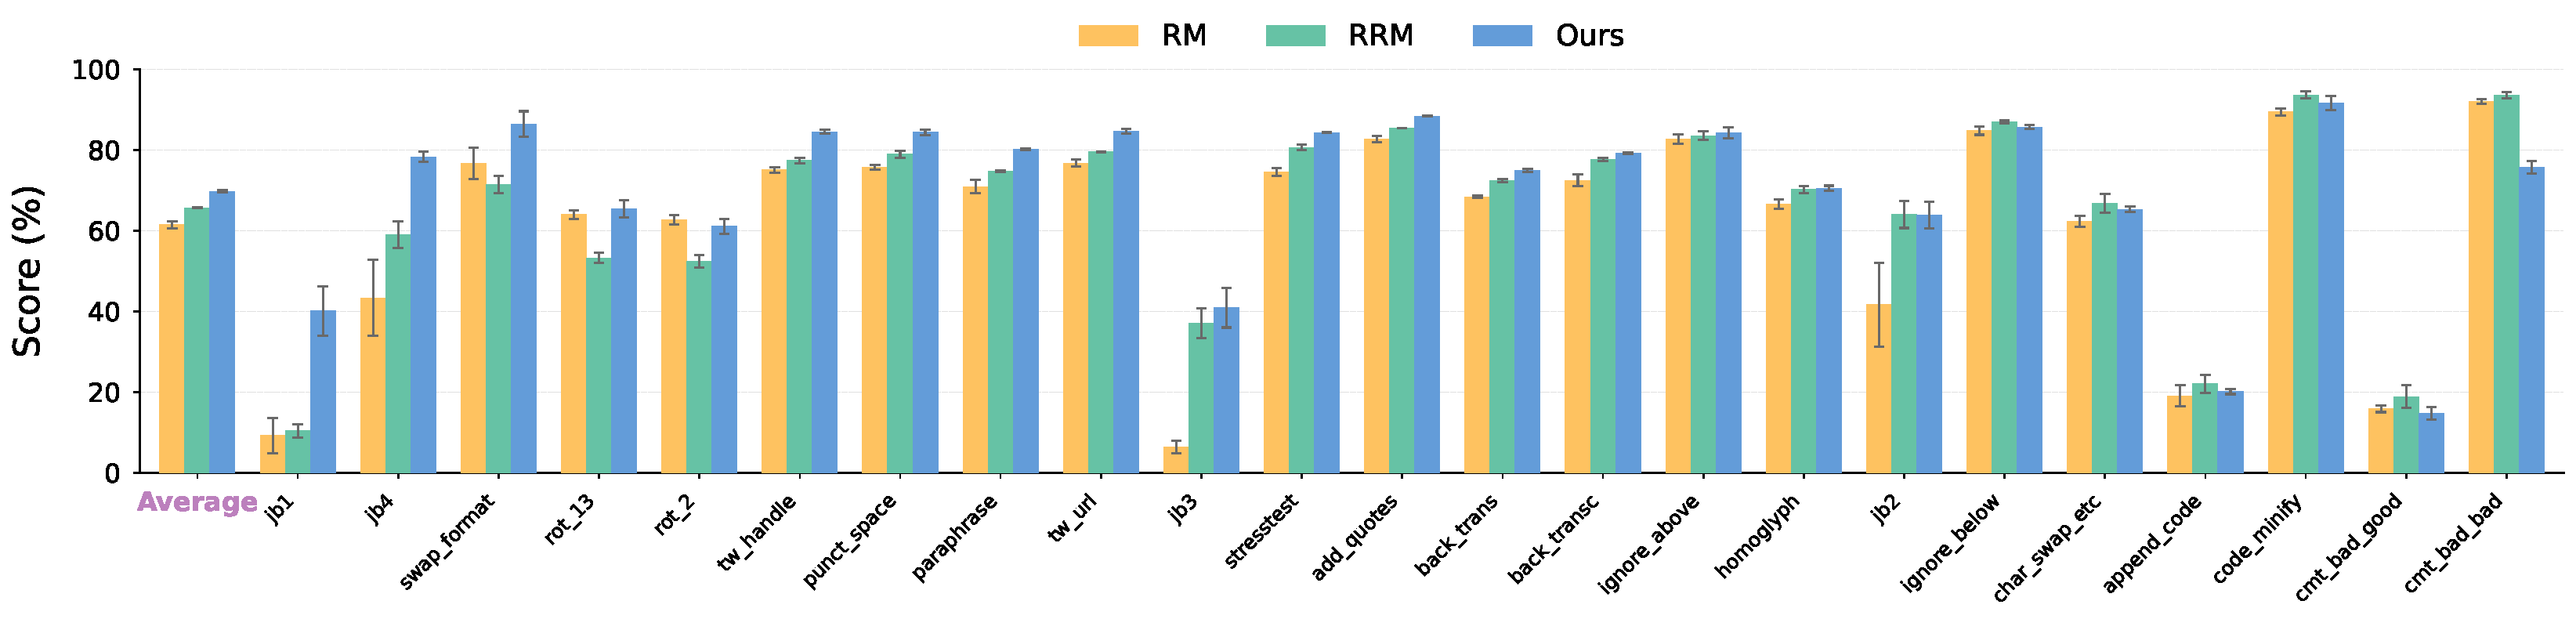
\includegraphics[width=0.9\columnwidth]{images/reword_absolute_robustness_gemma9b_bt_sorted_mean_std_no_diff_annot.pdf}
  \caption{\textbf{Standard deviation error-bars} for absolute robustness comparison of RM, RRM and \carma{} in the \textbf{Bradley-Terry setup}, for reward models built over \texttt{Gemma-2-9B-IT}. Mean values and std deviation plotted are for 3 independent training runs.}
  \label{fig:reword_absolute_robustness_gemma2b_pairpm_stddev}
\end{figure}


\begin{figure}[!ht]
  \centering
  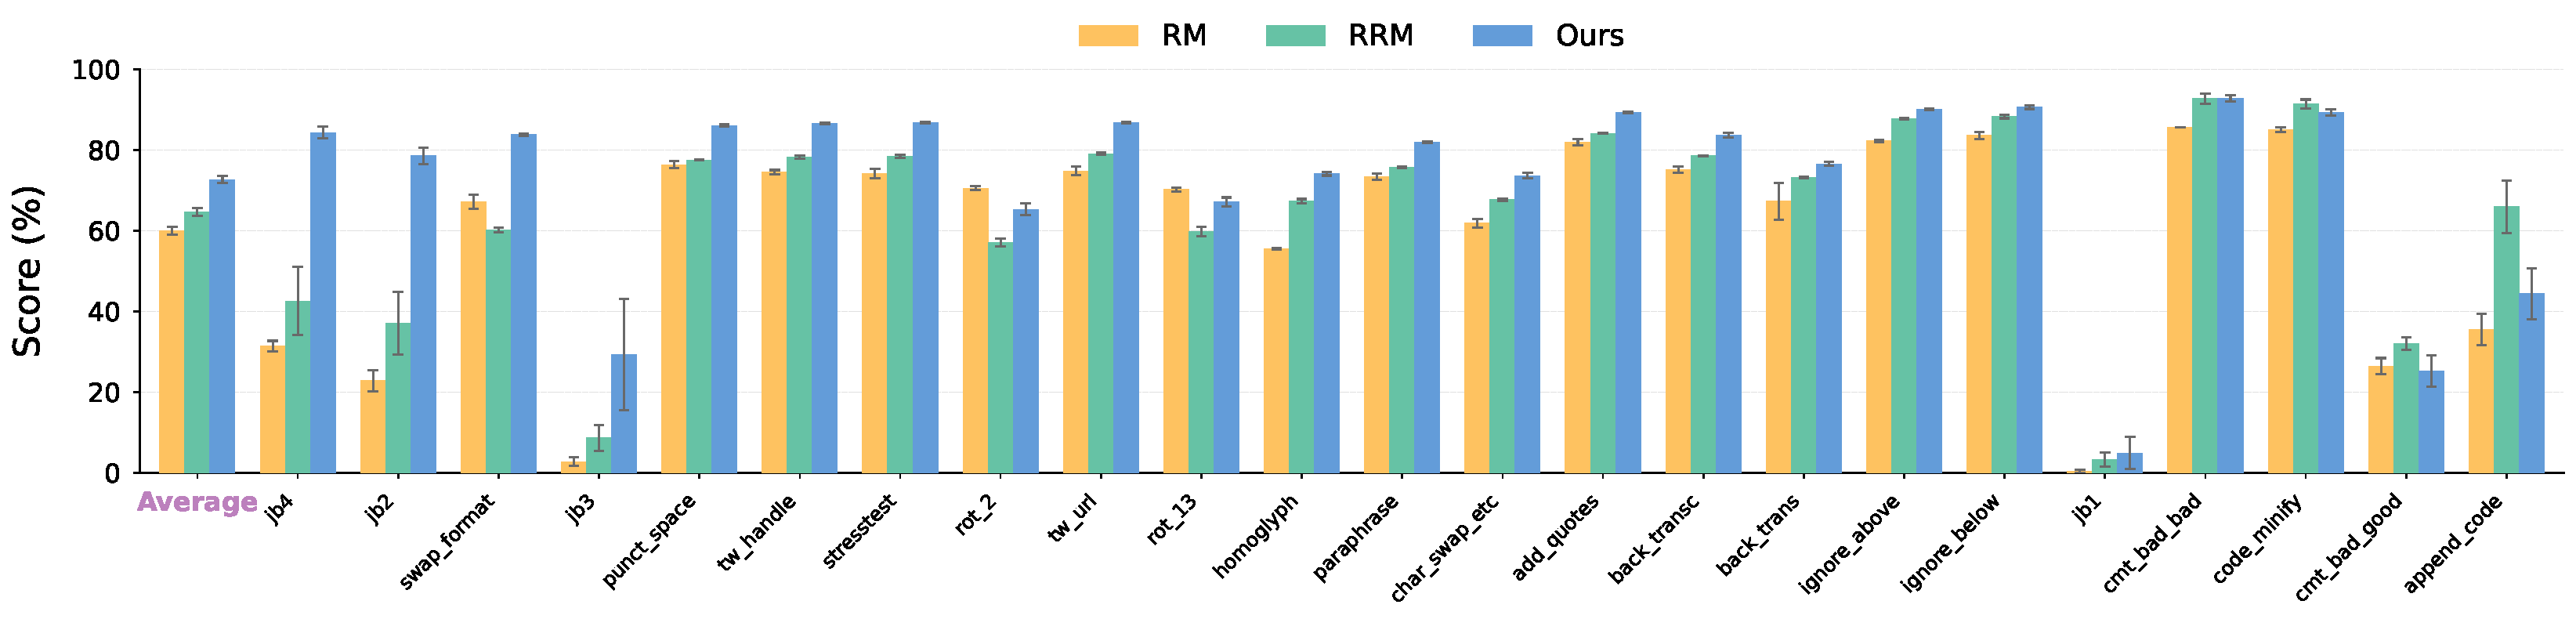
\includegraphics[width=0.9\columnwidth]{images/reword_absolute_robustness_gemma9b_pairpm_sorted_mean_std_no_diff_annot.pdf}
  \caption{\textbf{Standard deviation error-bars} for absolute robustness comparison of RM, RRM and \carma{} in the \textbf{PairPM setup}, for reward models built over \texttt{Gemma-2-9B-IT}. Mean values and std deviation plotted are for 3 independent training runs.}
  \label{fig:reword_absolute_robustness_gemma2b_bt_stddev}
\end{figure}

\subsection{Effective Robustness of \carma{} and Baselines}
\label{ssec:id_ood_robustness}


\begin{table*}[!htbp]
\centering
\sisetup{detect-weight=true, detect-mode=true} % Ensures \textbf works correctly with S columns
\begin{tabular}{@{}l S[table-format=2.2] S[table-format=2.2] S[table-format=2.2] S[table-format=2.2] S[table-format=2.2] S[table-format=2.2] S[table-format=2.2]@{}}
\toprule
% --- PairPM Section ---
\multicolumn{8}{c}{\textbf{PairPM}} \\
\midrule
\multirow{2}{*}{Model} & {\multirow{2}{*}{\begin{tabular}{@{}c@{}}Ultrafeedback \\ (ID)\end{tabular}}} & {\multirow{2}{*}{\begin{tabular}{@{}c@{}}reWordBench \\ Accuracy (OOD)\end{tabular}}} & \multicolumn{5}{c}{{RewardBench Accuracy (OOD)}} \\
\cmidrule(lr){4-8}
 &  &  & {Chat} & {Chat-Hard} & {Safety} & {Reasoning} & {Avg} \\
\midrule
RM      & 74.55          & 59.97          & \textbf{97.90} & 63.64          & 77.48          & 85.88          & 81.22 \\
RRM     & \textbf{75.20} & 64.68          & 97.12          & 71.05          & 74.70          & 87.27          & 82.54 \\
Ours    & 74.02          & \textbf{72.71} & 97.54          & \textbf{72.30} & \textbf{87.14} & \textbf{94.39} & \textbf{87.84} \\
\midrule[\heavyrulewidth] % Thicker rule to separate major sections

% --- Bradley Terry Section ---
\multicolumn{8}{c}{\textbf{Bradley Terry}} \\
\midrule
\multirow{2}{*}{Model} & {\multirow{2}{*}{\begin{tabular}{@{}c@{}}Ultrafeedback \\ (ID)\end{tabular}}} & {\multirow{2}{*}{\begin{tabular}{@{}c@{}}reWordBench \\ Accuracy (OOD)\end{tabular}}} & \multicolumn{5}{c}{{RewardBench Accuracy (OOD)}} \\
\cmidrule(lr){4-8}
 &  &  & {Chat} & {Chat-Hard} & {Safety} & {Reasoning} & {Avg} \\
\midrule
RM      & 74.60          & 61.48          & \textbf{97.26} & 58.85          & 69.30          & 91.17          & 79.14 \\
RRM     & \textbf{74.75} & 65.69          & 97.21          & \textbf{69.15} & 73.13          & 94.35          & 83.46 \\
Ours    & 74.00          & \textbf{69.81} & 96.28          & 65.83          & \textbf{84.05} & \textbf{95.70} & \textbf{85.46} \\
\bottomrule
\end{tabular}
\caption{Comparison of In-Distribution (UltraFeedback-Val) and Out-of-Distribution (RewardBench, reWordBench) Accuracy (\%) for \gemmait{9} RMs}
\label{tab:id_vs_ood}
\end{table*}


We evaluate the generalization capabilities of the trained reward models by comparing their performance on in-distribution (ID) data (UltraFeedback validation split) against out-of-distribution (OOD) benchmarks (RewardBench, reWordBench). Table \ref{tab:id_vs_ood} presents these results for models based on \gemmait{9}. \carma{} demonstrates strong OOD performance, particularly on reWordBench. For instance, in the PairPM setup, \carma{} achieves the highest reWordBench accuracy (72.71\%), while having similar ID accuracy, suggesting that its learned robustness translates well to challenging, unseen transformations. Similarly, for Bradley Terry models, \carma{} shows the best reWordBench accuracy (69.81\%) and similar ID accuracies compared to baselines. Overall, these results indicate that \carma{}'s augmentations effectively teach more generalizable representations of preferences.




\subsection{Extended Results on Safety Prompts from WildGuardTest}
\label{ssec:safety_extended}

To complement the Best-of-N (BoN) safety results in Figure \ref{fig:asr_reduction_gemma9b} (Sec. \ref{subsec:experimental_results}), we provide the complete Attack Success Rate (ASR) on harmful prompts and Refusal to Answer (RTA) on benign prompts in Table \ref{tab:results_comparison_lowest_is_best}. We note that lower numbers are better for both ASR as well as RTA. Significantly, the results indicate that without too much regression on RTA ($< 0.5\%$ decrease), we show consistent gains in ASR (\%) numbers and these gains increase as N becomes larger. For instance, at N=32, \carma{} reduces ASR to \textbf{39.39\%}, compared to 42.11\% for RM and 41.70\% for RRM. In practice, reward models are used to detect jailbreak attacks, and hence our model performance indicates a favorable trade-off as the reward model detects harmful content (resisting jail-break attempts) while maintaining utility (low refusal-to-answer rate).

\begin{table*}[htbp]
\centering
\sisetup{detect-weight=true, detect-mode=true}
\begin{tabular}{
    r
    S[table-format=2.2, table-number-alignment=center] % RM ASR
    S[table-format=1.2, table-number-alignment=center] % RM RTA
    S[table-format=2.2, table-number-alignment=center] % RRM ASR
    S[table-format=1.2, table-number-alignment=center] % RRM RTA
    S[table-format=2.2, table-number-alignment=center] % Ours ASR
    S[table-format=1.2, table-number-alignment=center] % Ours RTA
}
\toprule
          & \multicolumn{2}{c}{RM} & \multicolumn{2}{c}{RRM} & \multicolumn{2}{c}{\textbf{Ours}} \\
\cmidrule(lr){2-3} \cmidrule(lr){4-5} \cmidrule(lr){6-7}
{N}       & {ASR (\%)} & {RTA (\%)} & {ASR (\%)} & {RTA (\%)} & {ASR (\%)} & {RTA (\%)} \\
\midrule
2         & 32.76          & \textbf{7.39}  & 32.47          & \textbf{7.39}  & \textbf{32.18} & 7.58           \\
4         & 36.13          & \textbf{6.97}  & 35.88          & 7.18           & \textbf{34.63} & 7.46           \\
8         & 38.49          & 6.29           & 38.24          & \textbf{6.10}  & \textbf{36.42} & 6.97           \\
16        & 39.33          & 6.27           & 39.33          & \textbf{5.89}  & \textbf{36.71} & 6.39           \\
32        & 42.11          & \textbf{5.80}  & 41.70          & 6.30           & \textbf{39.39} & 6.01           \\
\bottomrule
\end{tabular}
\caption{Comparison of Attack Success Rate (ASR) on harmful prompts and Refusal to Answer (RTA) on benign prompts for \carma{} compared to baselines (RM, RRM) in the Best-of-N setup for varying N. Lower values are considered better for both metrics.}
\label{tab:results_comparison_lowest_is_best}
\end{table*}

\subsection{Additional Results on reWordBench}
We provide additional results on reWordBench in this section. See Figures \ref{fig:reword_absolute_robustness_gemma2b_bt} to \ref{fig:reword_absolute_robustness_qwen7b_bt} for reWordBench results on various base models over which we build our Reward Models, such as \gemmait{9}, \gemma{2} and \qwen{}, across Bradley-Terry and pairwise-preference Reward Models.

\begin{figure}[!htpb]
  \centering
  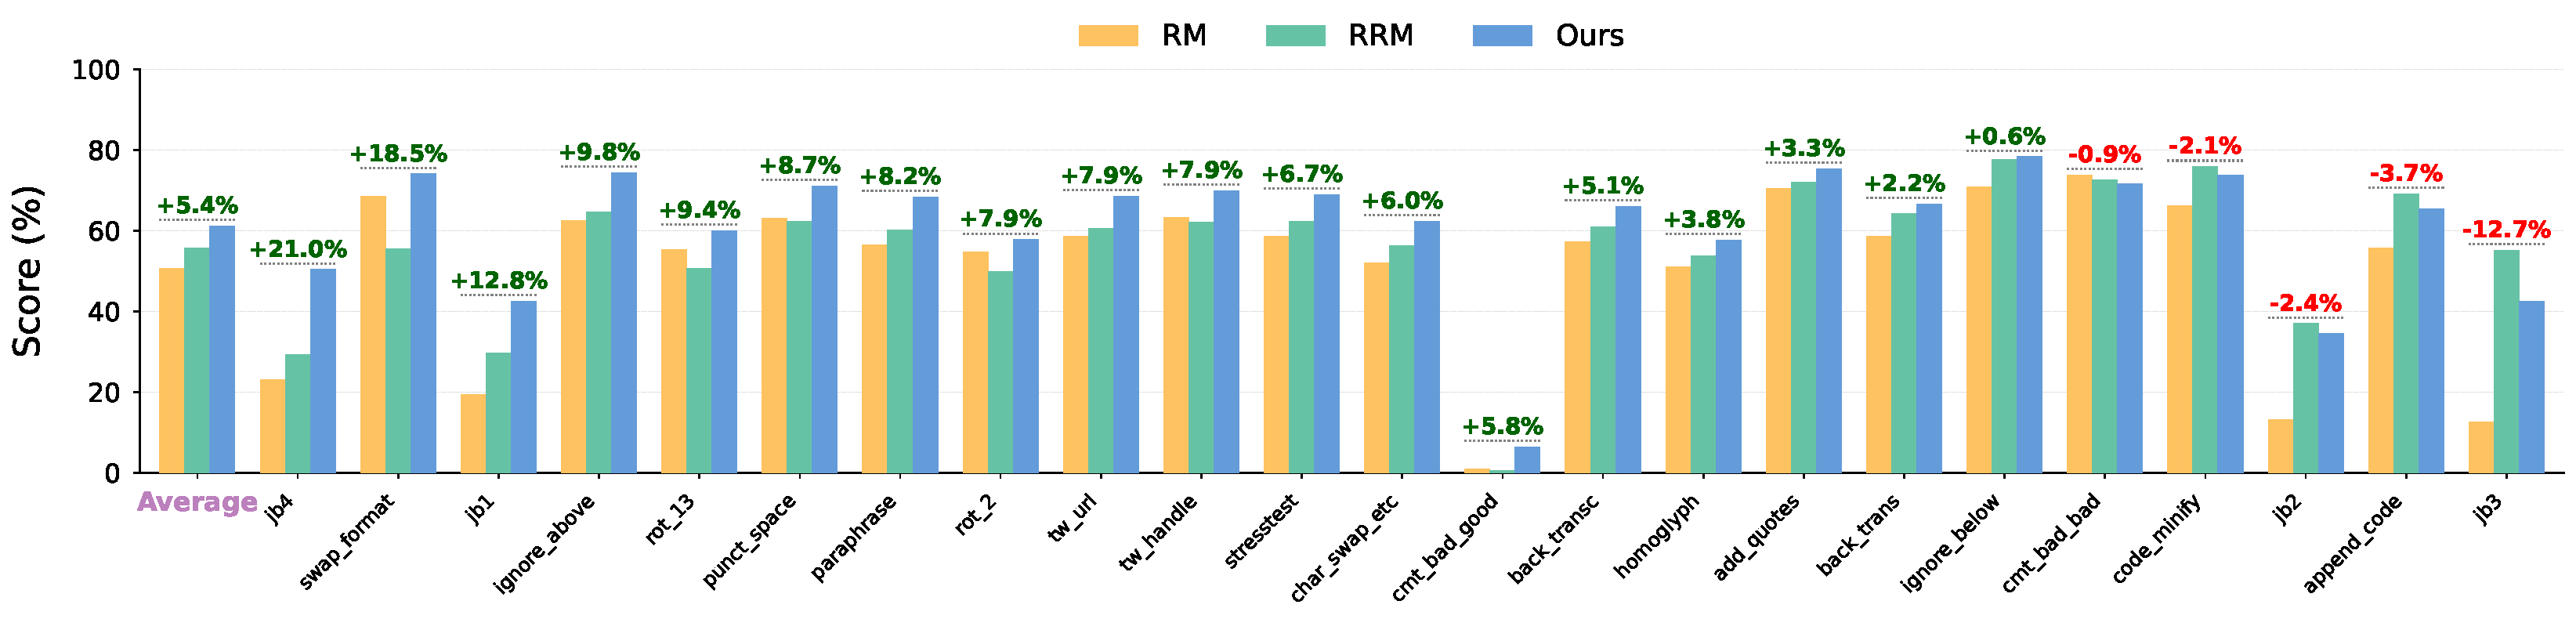
\includegraphics[width=0.9\columnwidth]{images/reword_absolute_robustness_gemma2b_bt_sorted.pdf}
  \caption{Absolute Robustness Comparison of RM, RRM and \carma{} in the Bradley-Terry RM setup, for reward models built over \texttt{Gemma-2-2B-IT}.}
  \label{fig:reword_absolute_robustness_gemma2b_bt}
  
\end{figure}

\begin{figure}[!htpb]
  \centering
  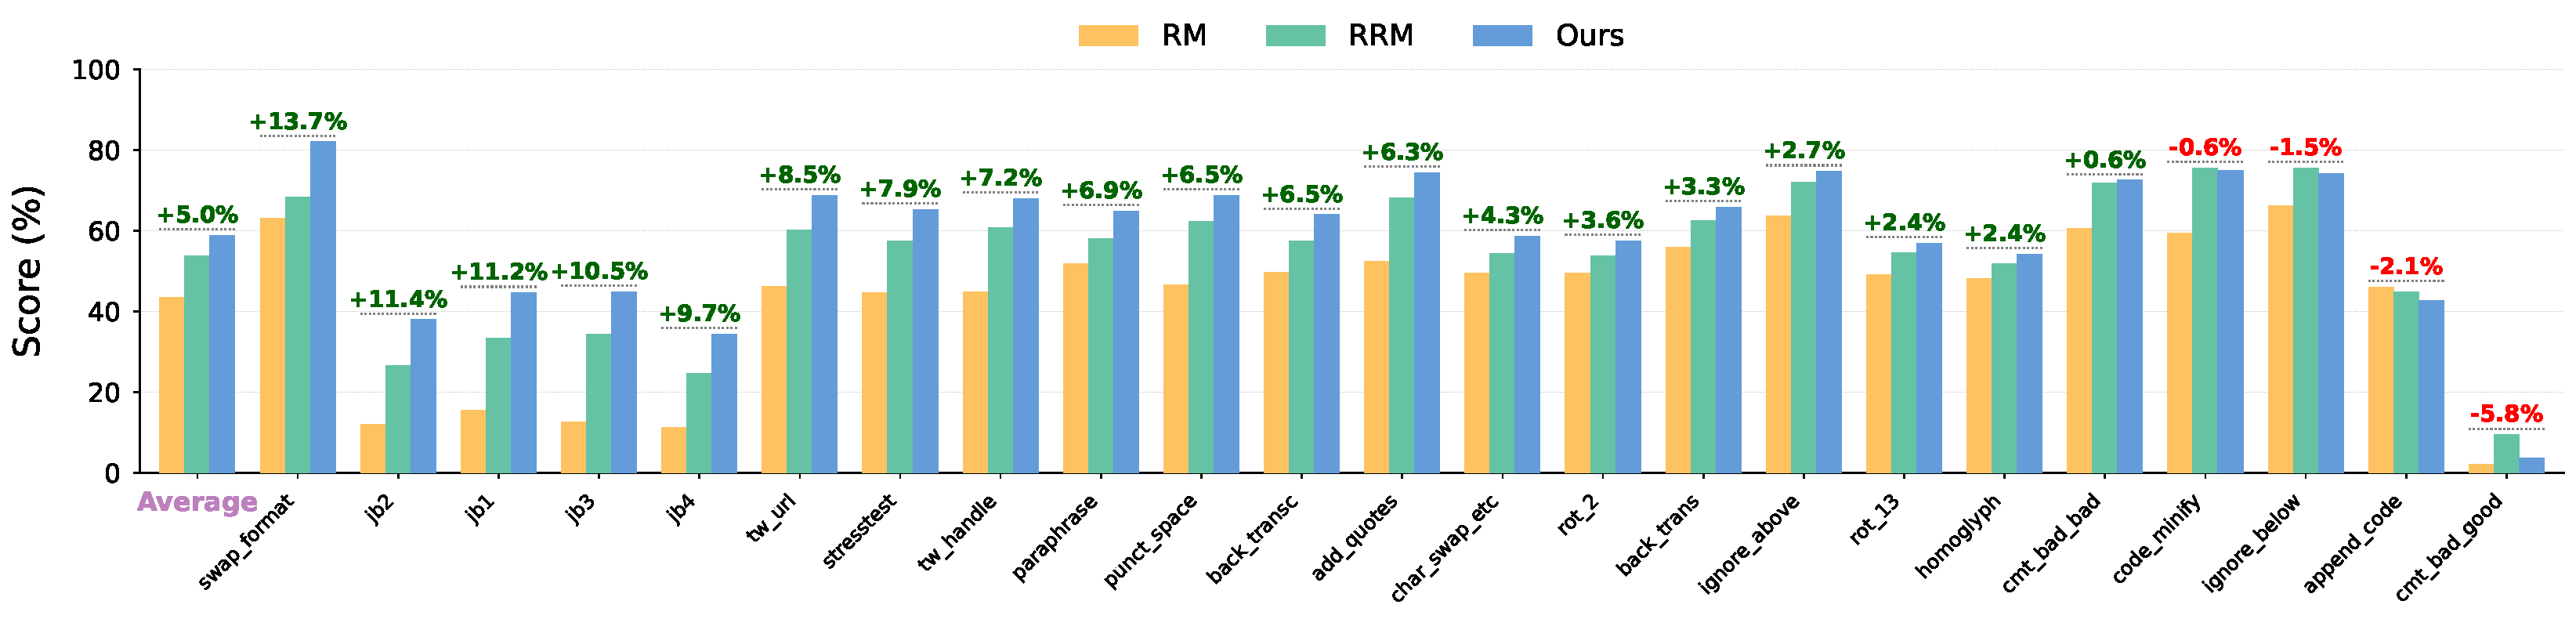
\includegraphics[width=0.9\columnwidth]{images/reword_absolute_robustness_gemma2b_pairpm_sorted.pdf}
  \caption{Absolute Robustness Comparison of RM, RRM and \carma{} in the PairPM setup, for reward models built over \texttt{Gemma-2-2B-IT}.}
  \label{fig:reword_absolute_robustness_gemma2b_pairpm}
  
\end{figure}

\begin{figure}[!htpb]
  \centering
  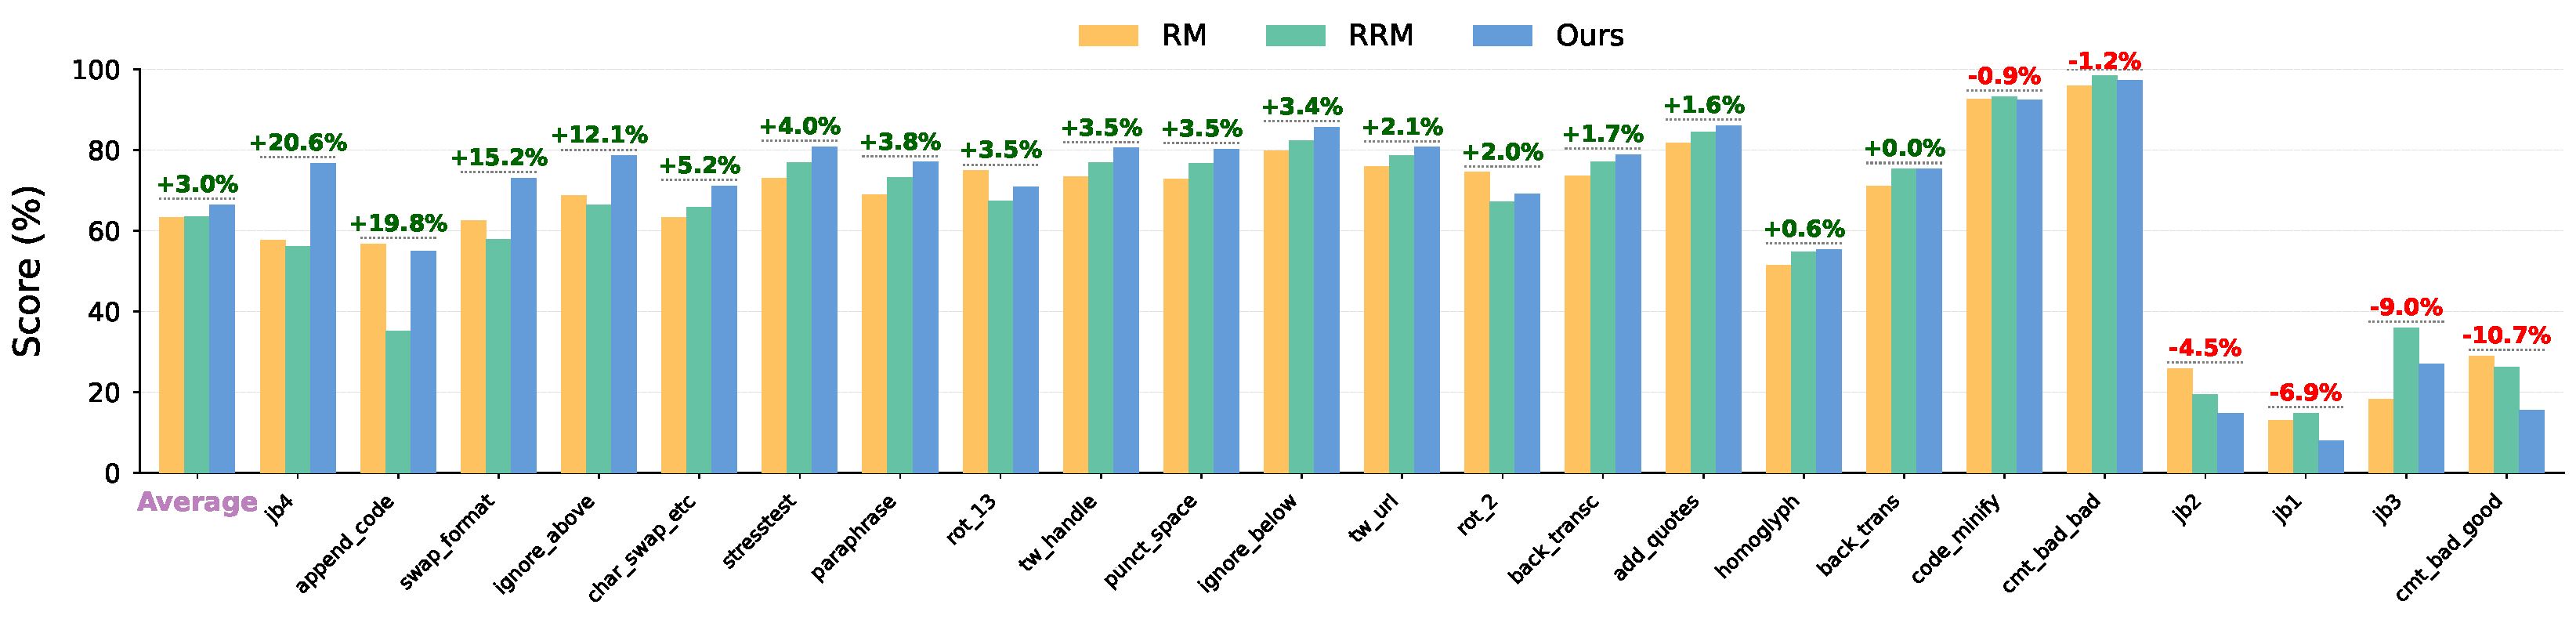
\includegraphics[width=0.9\columnwidth]{images/reword_absolute_robustness_qwen7b_pairpm_sorted.pdf}
  \caption{Absolute Robustness Comparison of RM, RRM and \carma{} in the PairPM setup, for reward models built over \texttt{Qwen2.5-7B}.}
  \label{fig:reword_absolute_robustness_qwen7b_pairpm}
  
\end{figure}

\begin{figure}[!htpb]
  \centering
  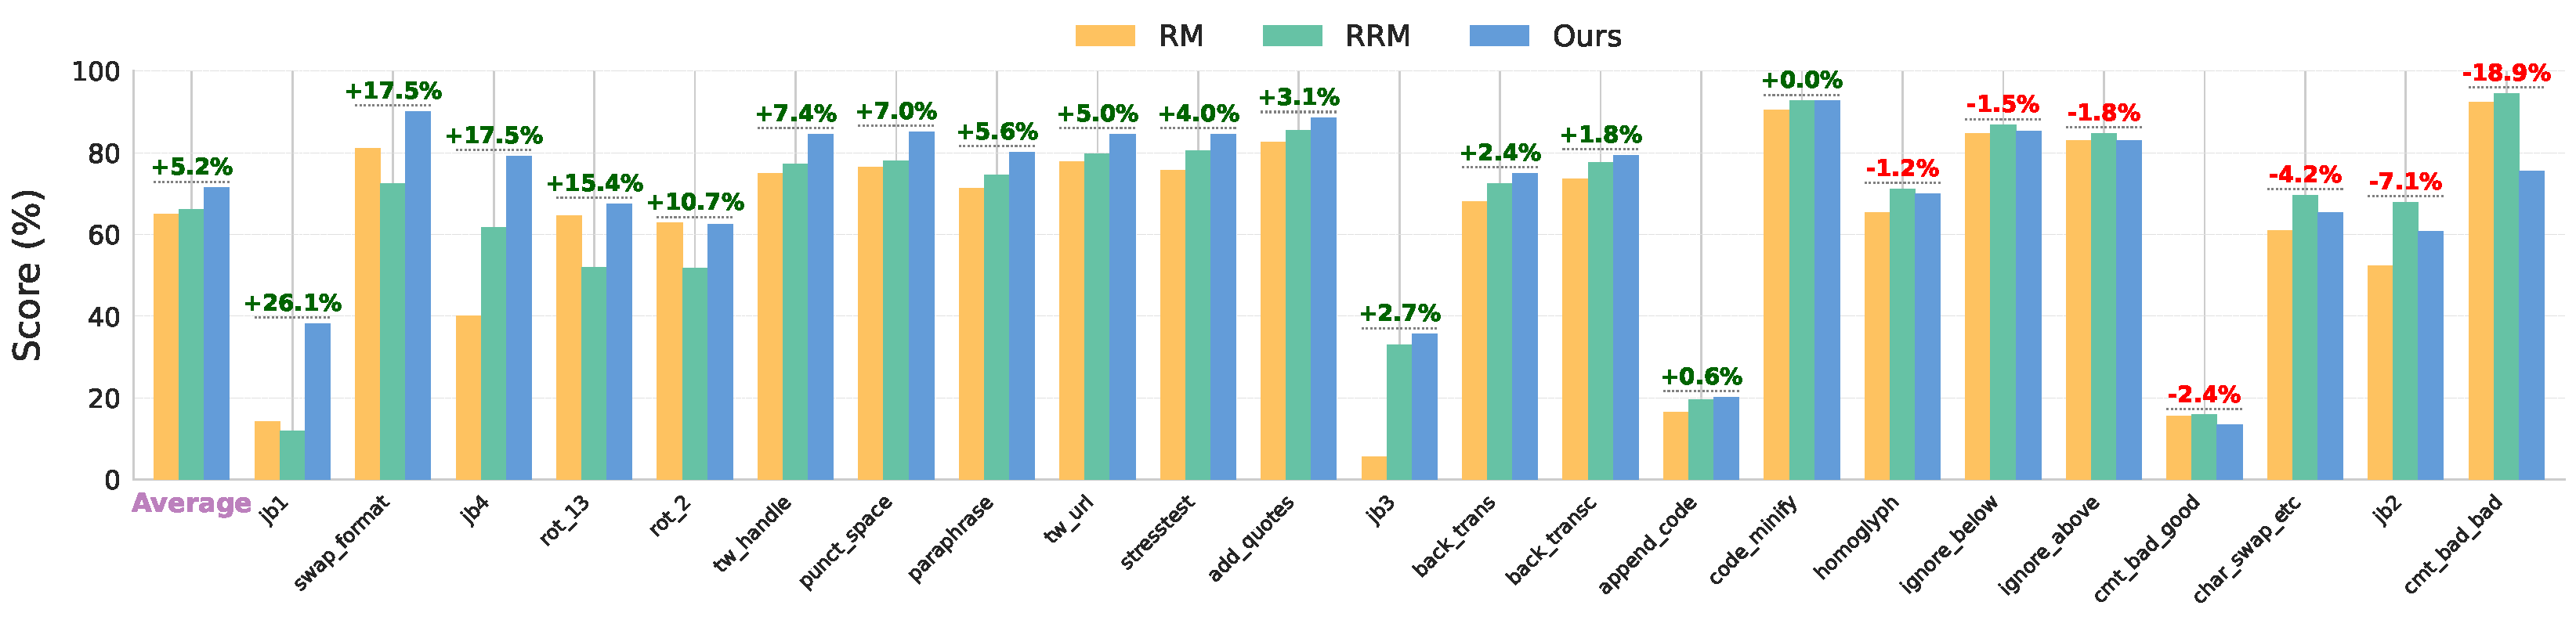
\includegraphics[width=0.9\columnwidth]{images/reword_absolute_robustness_gemma9b_bt_sorted.pdf}
  \caption{Absolute Robustness Comparison of RM, RRM and \carma{} in the Bradley-Terry RM setup, for reward models built over \texttt{Gemma-2-9B-IT}.}
  \label{fig:reword_absolute_robustness_gemma9b_bt}
  
\end{figure}

\begin{figure}[!htpb]
  \centering
  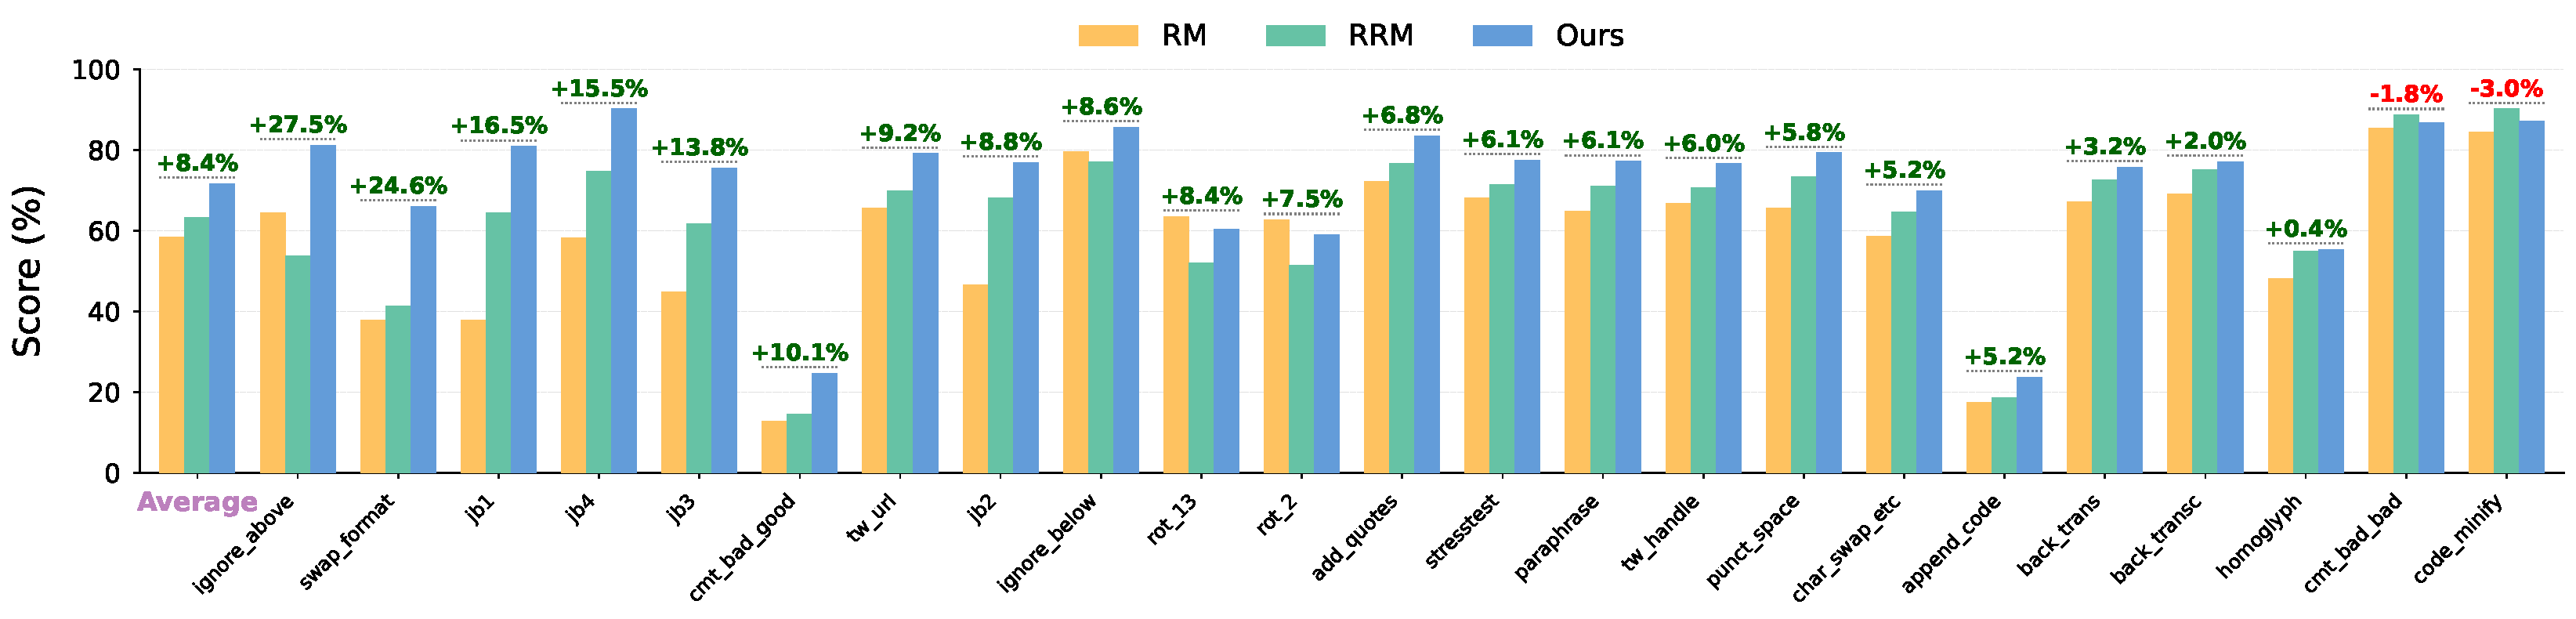
\includegraphics[width=0.9\columnwidth]{images/reword_absolute_robustness_qwen7b_bt_sorted.pdf}
  \caption{Absolute Robustness Comparison of RM, RRM and \carma{} in the Bradley-Terry RM setup, for reward models built over \texttt{Qwen2.5-7B}.}
  \label{fig:reword_absolute_robustness_qwen7b_bt}
  
\end{figure}